\documentclass[11pt,a4paper]{article}

\usepackage[top=2.5cm,bottom=2.5cm,left=2cm,right=2cm]{geometry}
\usepackage{amsmath,amssymb,booktabs}
\usepackage{hyperref}
\usepackage{pgfplots}
\pgfplotsset{compat=1.18}

\title{\textbf{Hydrogen Ground-State Hyperfine Splitting as a Canonical Activation Gap:\\
From the Fermi Contact Interaction to the Schottky Heat-Capacity Anomaly}}
\author{Omar Iskandarani\\
\small Independent Researcher, Groningen, The Netherlands\\
\small \href{mailto:info@omariskandarani.com}{info@omariskandarani.com}\quad ORCID: 0009-0006-1686-3961}
\date{March 2026}

\begin{document}
    \maketitle
    
    \begin{abstract}
        We give a self-contained, orthodox derivation of the hydrogen $1s$ hyperfine splitting starting from the magnetic dipole field (including its distributional contact term) and the resulting Fermi contact Hamiltonian. The leading-order gap $\Delta E_{\mathrm{hfs}}$ is expressed in standard constants, recovering the well-known scaling $\Delta E_{\mathrm{hfs}}\propto \alpha^4(m_e/m_p)m_ec^2$. We then treat the $(F=0)$--$(F=1)$ manifold as a two-level system with degeneracies $(g_0,g_1)=(1,3)$ and derive the exact canonical heat capacity (Schottky anomaly), including its low-temperature asymptotic and an explicit derivation of the peak condition for the degeneracy-asymmetric case. Numerical evaluation yields $\Delta E_{\mathrm{hfs}}\approx 5.88~\mu\mathrm{eV}$ from the leading term, to be compared with the experimental value $5.8743~\mu\mathrm{eV}$ (fractional error $\approx 0.097\%$), with the remaining discrepancy attributable to known QED, recoil, and proton-structure corrections.
    \end{abstract}
    
    \vspace{0.5cm}
    \noindent\textbf{Keywords:} hydrogen hyperfine structure; Fermi contact interaction; Schottky anomaly; two-level system; canonical ensemble; low-temperature thermodynamics; atomic spectroscopy.
    \vspace{0.5cm}

%======================================================================
    \section{Introduction}
        \label{sec:intro}
%======================================================================
        
        The hydrogen ground-state hyperfine splitting provides a concrete, experimentally calibrated example of a gapped two-level subsystem.
        Independently, the Schottky anomaly describes the characteristic heat-capacity peak arising from discrete-level occupation in the canonical ensemble.
        Both topics are standard, but they are often presented separately (atomic structure vs.\ thermal physics).
        The purpose of this manuscript is to present a single, fully explicit derivation chain that (i) derives the leading-order hyperfine gap from the Fermi contact interaction and (ii) propagates that gap into thermodynamic predictions for the two-level heat capacity, including an explicit derivation of the peak condition for the degeneracy-asymmetric case $(g_0,g_1)=(1,3)$.
        Accordingly, the contribution is pedagogical and synthetic rather than one of new fundamental physics:
        it provides a closed analytic-to-thermodynamic derivation chain from the hydrogen $1s$ hyperfine gap
        to the exact degeneracy-asymmetric Schottky anomaly, with explicit millikelvin scales relevant to low-temperature spectroscopy and thermodynamics.

%======================================================================
    \section{Definitions and standard identities}
        \label{sec:defs}
%======================================================================
        
        We use SI units. The fundamental constants are: $c$, $\hbar$, $h=2\pi\hbar$, $e$, $\varepsilon_0$, $\mu_0=1/(\varepsilon_0 c^2)$, $k_B$, and the electron and proton masses $(m_e,m_p)$.
        
        The fine-structure constant is
        \begin{equation}
            \alpha \equiv \frac{e^2}{4\pi\varepsilon_0 \hbar c}.
            \label{eq:alpha_def}
        \end{equation}
        
        The Bohr radius is
        \begin{equation}
            a_0 \equiv \frac{4\pi\varepsilon_0 \hbar^2}{m_e e^2}.
            \label{eq:a0_def1}
        \end{equation}
        Using \eqref{eq:alpha_def} (i.e.\ $e^2=4\pi\varepsilon_0\hbar c\,\alpha$), one obtains the standard identity
        \begin{equation}
            a_0=\frac{\hbar}{m_e c}\,\frac{1}{\alpha}.
            \label{eq:a0_def2}
        \end{equation}
        
        The electron and proton magnetic moments are written using $g$-factors:
        \begin{equation}
            \boldsymbol{\mu}_e = -g_e \mu_B \frac{\mathbf{S}}{\hbar},\qquad
            \boldsymbol{\mu}_p = +g_p \mu_N \frac{\mathbf{I}}{\hbar},
            \label{eq:moments_def}
        \end{equation}
        where $\mathbf{S}$ is the electron spin operator and $\mathbf{I}$ is the proton spin operator, and
        \begin{equation}
            \mu_B \equiv \frac{e\hbar}{2m_e},\qquad
            \mu_N \equiv \frac{e\hbar}{2m_p}.
            \label{eq:muB_muN}
        \end{equation}
        For hydrogen $1s$, we use $g_e\simeq 2$ and $g_p\simeq 5.5856947$ (proton $g$-factor) for the leading-order estimate; the effect of using the free-electron value $g_e=2.002319304\ldots$ is discussed in Section~\ref{sec:numerics} \cite{CODATA2022}.
        
        The normalized $1s$ wavefunction is
        \begin{equation}
            \psi_{1s}(\mathbf{r})=\frac{1}{\sqrt{\pi a_0^3}}e^{-r/a_0},
            \qquad
            |\psi_{1s}(0)|^2=\frac{1}{\pi a_0^3}.
            \label{eq:psi0}
        \end{equation}

%======================================================================
    \section{Magnetic dipole interaction and the Fermi contact term}
        \label{sec:fermi}
%======================================================================
        
        \subsection{Dipole field and contact contribution}
            The magnetic field of a point dipole $\boldsymbol{\mu}$ at the origin contains a distributional (contact) term.
            In SI units one may write \cite{Jackson1999}
            \begin{equation}
                \mathbf{B}(\mathbf{r})
                =
                \frac{\mu_0}{4\pi r^3}\Bigl[3\hat{\mathbf{r}}(\boldsymbol{\mu}\cdot\hat{\mathbf{r}})-\boldsymbol{\mu}\Bigr]
                +\frac{2\mu_0}{3}\,\boldsymbol{\mu}\,\delta^{(3)}(\mathbf{r}).
                \label{eq:B_dipole_contact}
            \end{equation}
            For an $s$-state, the isotropic contact term is the relevant contribution to the hyperfine splitting.
        
        \subsection{Fermi contact Hamiltonian and consistent sign convention}
            To avoid sign ambiguity, we compute the interaction as the energy of the electron magnetic moment
            in the proton's magnetic field:
            \begin{equation}
                H_{\mathrm{contact}}
                =
                -\boldsymbol{\mu}_e\cdot \mathbf{B}_p^{(\mathrm{contact})}.
            \end{equation}
            Using the proton contact field from \eqref{eq:B_dipole_contact},
            \begin{equation}
                \mathbf{B}_p^{(\mathrm{contact})}
                =
                \frac{2\mu_0}{3}\,\boldsymbol{\mu}_p\,\delta^{(3)}(\mathbf{r}),
            \end{equation}
            we obtain
            \begin{equation}
                H_{\mathrm{contact}}
                =
                -\frac{2\mu_0}{3}\,(\boldsymbol{\mu}_e\cdot \boldsymbol{\mu}_p)\,\delta^{(3)}(\mathbf{r}).
                \label{eq:H_contact_start}
            \end{equation}
            
            The electron and proton magnetic moments are
            \begin{equation}
                \boldsymbol{\mu}_e = -g_e \mu_B \frac{\mathbf{S}}{\hbar},
                \qquad
                \boldsymbol{\mu}_p = +g_p \mu_N \frac{\mathbf{I}}{\hbar},
                \label{eq:moments_def_repeat}
            \end{equation}
            so that
            \begin{equation}
                \boldsymbol{\mu}_e\cdot \boldsymbol{\mu}_p
                =
                -\,g_e g_p\,\mu_B\mu_N\,\frac{\mathbf{S}\cdot \mathbf{I}}{\hbar^2}.
            \end{equation}
            Substituting into \eqref{eq:H_contact_start} gives
            \begin{equation}
                H_{\mathrm{contact}}
                =
                +\frac{2\mu_0}{3}\,g_e g_p\,\mu_B\mu_N\,
                \frac{\mathbf{S}\cdot\mathbf{I}}{\hbar^2}\,\delta^{(3)}(\mathbf{r}).
                \label{eq:H_Fermi_SI}
            \end{equation}
            
            Taking the expectation value in the $1s$ spatial state yields
            \begin{equation}
                \langle H_{\mathrm{contact}}\rangle_{1s}
                =
                A\,\mathbf{S}\cdot\mathbf{I},
                \qquad
                A
                \equiv
                \frac{2\mu_0}{3}\,g_e g_p\,\mu_B\mu_N\,
                \frac{|\psi_{1s}(0)|^2}{\hbar^2},
                \label{eq:A_def}
            \end{equation}
            with $A>0$.
            
            The energy eigenstates are labeled by total spin $\mathbf{F}=\mathbf{S}+\mathbf{I}$ with $S=I=1/2$ and $F\in\{0,1\}$.
            Using
            \begin{equation}
                \mathbf{S}\cdot\mathbf{I}
                =
                \frac{1}{2}\Bigl(F(F+1)-S(S+1)-I(I+1)\Bigr)\hbar^2,
                \label{eq:SdotI}
            \end{equation}
            and $S(S+1)=I(I+1)=3/4$, one finds
            \begin{equation}
                \langle \mathbf{S}\cdot\mathbf{I}\rangle_{F=1}=+\frac{1}{4}\hbar^2,
                \qquad
                \langle \mathbf{S}\cdot\mathbf{I}\rangle_{F=0}=-\frac{3}{4}\hbar^2.
            \end{equation}
            
            Define
            \begin{equation}
                \mathcal{A}\equiv A\hbar^2
                =
                \frac{2\mu_0}{3}\,g_e g_p\,\mu_B\mu_N\,|\psi_{1s}(0)|^2.
                \label{eq:Acal_def}
            \end{equation}
            Then
            \begin{equation}
                \Delta E_{\mathrm{hfs}}
                \equiv
                E_{F=1}-E_{F=0}
                =
                \mathcal{A}\left(\frac{1}{4}-\left(-\frac{3}{4}\right)\right)
                =
                \mathcal{A}.
                \label{eq:DeltaE_A}
            \end{equation}
            Since $\mathcal{A}>0$, the singlet lies below the triplet, and therefore
            \[
                E_{F=0}<E_{F=1},
                \qquad
                \Delta E_{\mathrm{hfs}}>0.
            \]
            
            Substituting $|\psi_{1s}(0)|^2=1/(\pi a_0^3)$ and the definitions of $\mu_B,\mu_N$ yields the standard leading-order Fermi-contact formula
            \begin{equation}
                \Delta E_{\mathrm{hfs}}
                =
                \frac{2\mu_0}{3}\,g_e g_p\,\mu_B\mu_N\,\frac{1}{\pi a_0^3}.
                \label{eq:DeltaE_SI_form}
            \end{equation}
            For a closely related pedagogical derivation and sign-consistent discussion, see Griffiths \cite{GriffithsAJP1982}.

%======================================================================
    \section{Closed-form expression in \texorpdfstring{$\alpha$}{alpha}}
        \label{sec:closedform}
%======================================================================
        
        We eliminate $\mu_0,\mu_B,\mu_N,a_0$ in favor of $(\alpha,m_e,m_p,c)$.
        
        Use $\mu_0=1/(\varepsilon_0 c^2)$ and \eqref{eq:muB_muN}:
        \begin{equation}
            \mu_0\,\mu_B\mu_N
            =
            \frac{1}{\varepsilon_0 c^2}\left(\frac{e\hbar}{2m_e}\right)\left(\frac{e\hbar}{2m_p}\right)
            =
            \frac{e^2\hbar^2}{4\varepsilon_0 c^2\,m_e m_p}.
        \end{equation}
        Insert into \eqref{eq:DeltaE_SI_form}:
        \begin{equation}
            \Delta E_{\mathrm{hfs}}
            =
            \frac{g_e g_p}{6\pi}\,
            \frac{e^2\hbar^2}{\varepsilon_0 c^2\,m_e m_p\,a_0^3}.
            \label{eq:DeltaE_mid}
        \end{equation}
        Now eliminate $a_0$ using \eqref{eq:a0_def1}:
        \[
            a_0=\frac{4\pi\varepsilon_0\hbar^2}{m_e e^2}
            \quad\Longrightarrow\quad
            \frac{1}{a_0^3}=\left(\frac{m_e e^2}{4\pi\varepsilon_0\hbar^2}\right)^3.
        \]
        Substitute:
        \begin{align}
            \Delta E_{\mathrm{hfs}}
            &=
            \frac{g_e g_p}{6\pi}\,
            \frac{e^2\hbar^2}{\varepsilon_0 c^2\,m_e m_p}\,
            \left(\frac{m_e e^2}{4\pi\varepsilon_0\hbar^2}\right)^3
            \nonumber\\
            &=
            \frac{g_e g_p}{6\pi}\,
            \frac{m_e^2}{m_p}\,
            \frac{e^8}{(4\pi)^3\,\varepsilon_0^4\,\hbar^4}\,
            \frac{1}{c^2}.
            \label{eq:DeltaE_expand}
        \end{align}
        Using $e^2/(4\pi\varepsilon_0)=\alpha\hbar c$, one has
        \[
            \frac{e^8}{(4\pi)^3\varepsilon_0^4}
            =
            (4\pi)(\alpha\hbar c)^4,
        \]
        so that
        \begin{align}
            \Delta E_{\mathrm{hfs}}
            &=
            \frac{g_e g_p}{6\pi}\,
            \frac{m_e^2}{m_p}\,
            \frac{(4\pi)(\alpha\hbar c)^4}{\hbar^4 c^2}
            \nonumber\\
            &=
            \frac{4\pi}{6\pi}\,g_e g_p\,\alpha^4\left(\frac{m_e}{m_p}\right)m_e c^2
            =
            \frac{2}{3}\,g_e g_p\,\alpha^4\left(\frac{m_e}{m_p}\right)m_e c^2.
        \end{align}
        Thus the compact leading-order form is
        \begin{equation}
            \boxed{
                \Delta E_{\mathrm{hfs}}
                =
                \frac{2}{3}\,g_e g_p\,\alpha^4\left(\frac{m_e}{m_p}\right)\,m_e c^2.
            }
            \label{eq:DeltaE_alpha4}
        \end{equation}
        
        \paragraph{Literature note (prior derivations).}
            Equation~\eqref{eq:DeltaE_alpha4} is the standard leading-order Fermi-contact result (``Fermi energy'')
            and is derived in many classic sources (e.g.\ Berestetskii--Lifshitz--Pitaevskii) as well as modern reviews.
            We reproduce the algebra here to keep the manuscript self-contained and to connect the gap to the thermodynamic
            analysis below \cite{BLP_QED1982,Karshenboim2002}.

%======================================================================
    \section{Numerical evaluation and the 21 cm line}
    \label{sec:numerics}
%======================================================================
    
    \begin{table}[t]
        \centering
        \caption{Constants used in the leading-order numerical estimate of $\Delta E_{\mathrm{hfs}}^{(0)}$.}
        \label{tab:constants}
        \begin{tabular}{lll}
            \toprule
            Quantity & Value & Source \\
            \midrule
            $\alpha$ & $7.2973525643\times 10^{-3}$ & \cite{CODATA2022} \\
            $m_e c^2$ & $510998.950~\mathrm{eV}$ & \cite{CODATA2022} \\
            $m_e/m_p$ & $5.446170214\times 10^{-4}$ & \cite{CODATA2022} \\
            $g_e$ & $2$ (leading-order) & convention in this paper \\
            $g_p$ & $5.5856947$ & \cite{CODATA2022} \\
            \bottomrule
        \end{tabular}
    \end{table}
    
    Using CODATA constants and $g_p$ \cite{CODATA2022}, \eqref{eq:DeltaE_alpha4} gives a leading-order estimate
    \begin{equation}
        \Delta E_{\mathrm{hfs}}^{(0)} \approx 5.88~\mu\mathrm{eV}.
    \end{equation}
    Experimentally, the hydrogen ground-state hyperfine transition frequency is
    \begin{equation}
        \nu_{\mathrm{hfs}} = 1420.40575177~\mathrm{MHz},
    \end{equation}
    corresponding to
    \begin{equation}
        \Delta E_{\mathrm{hfs}}^{\mathrm{(exp)}} = h\nu_{\mathrm{hfs}} \approx 5.8743~\mu\mathrm{eV}.
        \label{eq:DeltaE_exp}
    \end{equation}
    (See primary measurement references such as Hellwig et al.\ \cite{Hellwig1970}.)
    
    \paragraph{Fractional deviation and input conventions.}
        Define
        \[
            \delta \equiv \frac{\Delta E_{\mathrm{hfs}}^{(0)}-\Delta E_{\mathrm{hfs}}^{\mathrm{(exp)}}}{\Delta E_{\mathrm{hfs}}^{\mathrm{(exp)}}}.
        \]
        Using the leading-order contact formula \eqref{eq:DeltaE_alpha4} with the conventional approximation $g_e\simeq 2$
        gives $\Delta E_{\mathrm{hfs}}^{(0)}\approx 5.88~\mu\mathrm{eV}$ and hence
        \[
            \delta \approx 9.7\times 10^{-4}\approx 0.097\%.
        \]
        If instead one inserts the free-electron value $g_e=2.002319304\ldots$ into the same leading-order expression,
        $\Delta E_{\mathrm{hfs}}^{(0)}$ shifts by $0.116\%$ and the residual changes at the $\sim 10^{-3}$ level.
        In precision theory one does not treat \eqref{eq:DeltaE_alpha4} as complete: radiative QED corrections,
        recoil effects, and proton-structure (Zemach-radius) contributions are required for ppm-level agreement
        \cite{Karshenboim2002,BLP_QED1982}.
        
        Define the gap temperature scale
        \begin{equation}
            T_\Delta \equiv \frac{\Delta E_{\mathrm{hfs}}^{\mathrm{(exp)}}}{k_B}\approx 68.17~\mathrm{mK}.
            \label{eq:TDelta}
        \end{equation}

%======================================================================
    \section{Thermodynamics: Schottky anomaly for the hyperfine doublet}
    \label{sec:schottky}
%======================================================================
    
    \subsection{Two-level system with degeneracy $(1,3)$}
        The $1s$ hyperfine manifold has a singlet ground state ($F=0$, degeneracy $g_0=1$)
        and a triplet excited state ($F=1$, degeneracy $g_1=3$).
        Treating the hyperfine degree of freedom as a two-level system with
        \begin{equation}
            E_0=0,\qquad E_1=\Delta E_{\mathrm{hfs}}^{\mathrm{(exp)}}\equiv \Delta,
        \end{equation}
        the partition function is
        \begin{equation}
            Z(\beta)=g_0 e^{-\beta E_0}+g_1 e^{-\beta E_1}
            =1+3e^{-\beta\Delta},
            \qquad
            \beta=\frac{1}{k_B T}.
            \label{eq:Z_hfs}
        \end{equation}
        The present treatment assumes that the hyperfine manifold can be regarded as an effectively isolated internal two-level subsystem,
        which is appropriate for dilute atomic hydrogen under conditions where spin-exchange collisions, molecular formation,
        and strong external-field splittings do not dominate the equilibration.
    
    \subsection{Exact heat capacity}
        The mean energy is
        \begin{equation}
            \langle E\rangle
            =
            \frac{3\Delta e^{-\beta\Delta}}{1+3e^{-\beta\Delta}}.
        \end{equation}
        Differentiation yields the exact Schottky heat capacity per atom:
        \begin{equation}
            \boxed{
                C_V(T)
                =
                k_B\left(\frac{\Delta}{k_B T}\right)^2
                \frac{3e^{-\Delta/(k_B T)}}{\left(1+3e^{-\Delta/(k_B T)}\right)^2}.
            }
            \label{eq:Cv_hfs}
        \end{equation}
        For one mole, multiply by Avogadro's number (replace $k_B$ by $R$) \cite{PathriaBeale2011,KittelKroemer1980}.
    
    \subsection{Low-temperature asymptotic (frozen regime)}
        For $k_B T\ll \Delta$, $e^{-\Delta/(k_B T)}\ll 1$ and \eqref{eq:Cv_hfs} reduces to
        \begin{equation}
            \boxed{
                C_V(T)\sim
                3k_B\left(\frac{\Delta}{k_B T}\right)^2 e^{-\Delta/(k_B T)}
                \qquad (k_B T\ll \Delta).
            }
            \label{eq:Cv_lowT}
        \end{equation}
        In the opposite limit $k_B T\gg \Delta$, the Boltzmann weights of the singlet and triplet levels become nearly equal,
        the internal entropy approaches $k_B\ln(g_0+g_1)=k_B\ln 4$, and the heat capacity again tends to zero:
        \begin{equation}
            C_V(T)\to 0 \qquad (T\to\infty).
        \end{equation}
        Thus the Schottky anomaly is localized in an intermediate temperature window around $T\sim T_\Delta$.
    
    \subsection{Peak location (derived) for general degeneracy ratio}
        Let $g_0$ be the ground-state degeneracy and $g_1$ the excited-state degeneracy, with gap $\Delta$.
        Define $r\equiv g_1/g_0$ and $x\equiv \beta\Delta=\Delta/(k_B T)$.
        Then
        \begin{equation}
            \frac{C_V}{k_B} = x^2\,\frac{r e^{-x}}{(1+r e^{-x})^2}.
            \label{eq:Cv_x}
        \end{equation}
        Let $y\equiv r e^{-x}$ so that $dy/dx=-y$. Writing $(C_V/k_B)=x^2\,y/(1+y)^2$, we obtain
        \begin{align}
            \frac{d}{dx}\left(\frac{C_V}{k_B}\right)
            &=
            2x\,\frac{y}{(1+y)^2}
            +
            x^2\,\frac{d}{dx}\left(\frac{y}{(1+y)^2}\right),
            \\[4pt]
            \frac{d}{dx}\left(\frac{y}{(1+y)^2}\right)
            &=
            \left(\frac{1}{(1+y)^2}-\frac{2y}{(1+y)^3}\right)\frac{dy}{dx}
            =
            \frac{(1-y)}{(1+y)^3}\,\frac{dy}{dx}.
        \end{align}
        Using $dy/dx=-y$ gives
        \begin{equation}
            \frac{d}{dx}\left(\frac{y}{(1+y)^2}\right)
            =
            -\frac{y(1-y)}{(1+y)^3}.
        \end{equation}
        Setting the derivative to zero yields the peak condition
        \begin{equation}
            \boxed{
                2(1+y)=x(1-y),
                \qquad y=r e^{-x}.
            }
            \label{eq:peak_condition}
        \end{equation}
        We do not claim originality for the transcendental peak equation itself; it is included here for completeness in the specific hydrogen-hyperfine context.
        For the physically relevant root one must have $y<1$, since the right-hand side of
        \eqref{eq:peak_condition} is positive only when $1-y>0$.
        For hydrogen hyperfine, $(g_0,g_1)=(1,3)$ so $r=3$. The solution of \eqref{eq:peak_condition}
        was obtained by standard one-dimensional root-finding (Newton or bisection), giving
        \begin{equation}
            x_{\mathrm{peak}}\equiv \frac{\Delta}{k_B T_{\mathrm{peak}}}\approx 2.8449,
            \qquad
            T_{\mathrm{peak}}\approx 0.3514\,T_\Delta \approx 24.0~\mathrm{mK}.
            \label{eq:Tpeak}
        \end{equation}
        At this point
        \[
            y_{\mathrm{peak}}=3e^{-x_{\mathrm{peak}}}\approx 3e^{-2.8449}\approx 0.175<1,
        \]
        so the positivity condition is self-consistently satisfied.
        At the peak one finds $C_V^{\max}\approx 1.02\,k_B$ per atom.
        
        \paragraph{Interpretation.}
            The hyperfine degree of freedom behaves thermodynamically as a discrete two-level subsystem:
            its contribution to $C_V$ is exponentially suppressed for $T\ll T_\Delta$, peaks near $T\sim 0.35\,T_\Delta$,
            and vanishes again for $T\gg T_\Delta$ as the two levels become nearly equally populated.
            
            \begin{figure}[t]
                \centering
                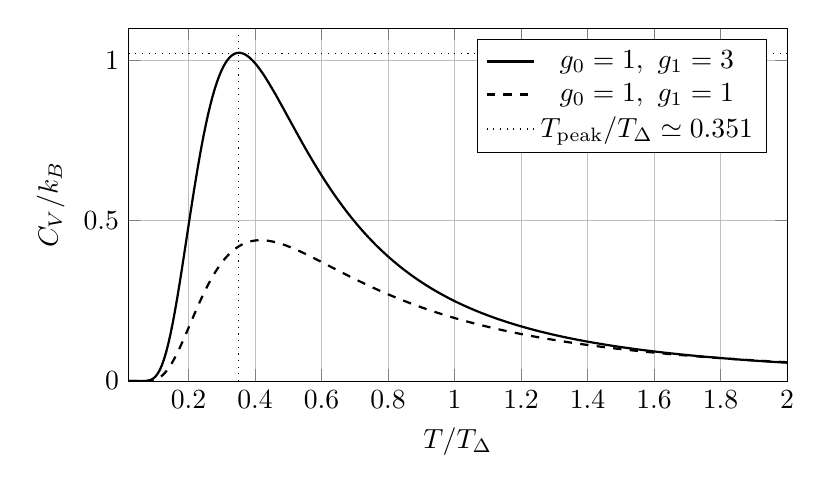
\begin{tikzpicture}
                    \begin{axis}[
                        width=0.82\textwidth,
                    height=0.5\textwidth,
                    xlabel={$T/T_\Delta$},
                    ylabel={$C_V/k_B$},
                    xmin=0.02, xmax=2.0,
                    ymin=0, ymax=1.1,
                    domain=0.02:2.0,
                    samples=300,
                    legend style={at={(0.97,0.97)},anchor=north east},
                    grid=both
                    ]
                        \addplot[thick]
                        {(1/x)^2 * (3*exp(-1/x)) / (1 + 3*exp(-1/x))^2};
                        \addlegendentry{$g_0=1,\ g_1=3$}
                        
                        \addplot[thick,dashed]
                        {(1/x)^2 * (exp(-1/x)) / (1 + exp(-1/x))^2};
                        \addlegendentry{$g_0=1,\ g_1=1$}
                        
                        \addplot[dotted] coordinates {(0.3514,0) (0.3514,1.1)};
                        \addplot[dotted] coordinates {(0,1.02) (2.0,1.02)};
                        \addlegendentry{$T_{\mathrm{peak}}/T_\Delta\simeq 0.351$}
                    \end{axis}
                \end{tikzpicture}
                \caption{
                    Dimensionless Schottky heat capacity $C_V/k_B$ versus reduced temperature $T/T_\Delta$
                    for the hydrogen hyperfine doublet $(g_0,g_1)=(1,3)$, compared with the symmetric two-level case $(g_0,g_1)=(1,1)$.
                    The asymmetric case peaks at $T_{\mathrm{peak}}/T_\Delta\simeq 0.351$ with $C_V^{\max}/k_B\simeq 1.02$,
                    whereas the symmetric case peaks at the larger temperature ratio $T/T_\Delta\simeq 0.417$.
                }
                \label{fig:schottky_hfs}
            \end{figure}

%======================================================================
    \section{Conclusion}
    \label{sec:conclusion}
%======================================================================
    
    We have presented a single self-contained derivation chain connecting the hydrogen $1s$ hyperfine splitting
    to the Schottky heat-capacity anomaly of the resulting two-level system.
    Starting from the dipole field with its contact term, we recovered the standard leading-order Fermi-contact gap
    and expressed it in closed form in terms of $\alpha$, $m_e$, $m_p$, and the spin $g$-factors.
    Using the experimentally measured hyperfine energy as the activation gap, we then derived the exact canonical
    heat capacity for the degeneracy-asymmetric $(g_0,g_1)=(1,3)$ system, including both low- and high-temperature limits
    and an explicit peak condition.
    The resulting millikelvin scale $T_\Delta$ and the peak temperature $T_{\mathrm{peak}}$ provide a direct bridge
    between atomic spectroscopy and low-temperature thermodynamics.
    Natural extensions include hydrogen-like ions, Zeeman-resolved hyperfine manifolds, and other discrete nuclear-spin systems.

%======================================================================
    \begin{thebibliography}{99}
        
        \bibitem{CODATA2022}
        E.~Tiesinga, P.~J.~Mohr, D.~B.~Newell, and B.~N.~Taylor (2023),
        \textit{The 2022 CODATA Recommended Values of the Fundamental Physical Constants},
        Rev.\ Mod.\ Phys.\ \textbf{95}, 025003.
        DOI: 10.1103/RevModPhys.95.025003.
        
        \bibitem{Jackson1999}
        J.~D.~Jackson (1999),
        \textit{Classical Electrodynamics}, 3rd ed.,
        Wiley. (Dipole field contact term; distributional $\delta$-term.)
        
        \bibitem{GriffithsAJP1982}
        D.~J.~Griffiths (1982),
        \textit{Hyperfine splitting in the ground state of hydrogen},
        Am.\ J.\ Phys.\ \textbf{50}, 698--703.
        DOI: 10.1119/1.12899.
        
        \bibitem{BLP_QED1982}
        V.~B.~Berestetskii, E.~M.~Lifshitz, and L.~P.~Pitaevskii (1982),
        \textit{Quantum Electrodynamics}, 2nd ed. (Course of Theoretical Physics, Vol.~4),
        Pergamon Press. (Fermi energy; hyperfine corrections.)
        
        \bibitem{Karshenboim2002}
        S.~G.~Karshenboim (2002),
        \textit{Hyperfine structure of the ground and first excited states in light hydrogen-like atoms},
        Eur.\ Phys.\ J.\ D \textbf{19}, 13--29.
        DOI: 10.1140/epjd/e20020045.
        
        \bibitem{Hellwig1970}
        H.~Hellwig, R.~F.~C.~Vessot, M.~W.~Levine, E.~M.~Mattison, D.~W.~Allan, and D.~J.~Glaze (1970),
        \textit{Measurement of the Unperturbed Hydrogen Hyperfine Transition Frequency},
        IEEE Trans.\ Instrum.\ Meas.\ \textbf{19}, 200--209.
        DOI: 10.1109/TIM.1970.4313902.
        
        \bibitem{PathriaBeale2011}
        R.~K.~Pathria and P.~D.~Beale (2011),
        \textit{Statistical Mechanics}, 3rd ed.,
        Elsevier. (Canonical fluctuation formula; two-level system.)
        
        \bibitem{KittelKroemer1980}
        C.~Kittel and H.~Kroemer (1980),
        \textit{Thermal Physics}, 2nd ed.,
        W.\ H.\ Freeman. (Schottky anomaly.)
    
    \end{thebibliography}

\end{document}